\documentclass[man]{apa6}
\usepackage{lmodern}
\usepackage{amssymb,amsmath}
\usepackage{ifxetex,ifluatex}
\usepackage{fixltx2e} % provides \textsubscript
\ifnum 0\ifxetex 1\fi\ifluatex 1\fi=0 % if pdftex
  \usepackage[T1]{fontenc}
  \usepackage[utf8]{inputenc}
\else % if luatex or xelatex
  \ifxetex
    \usepackage{mathspec}
  \else
    \usepackage{fontspec}
  \fi
  \defaultfontfeatures{Ligatures=TeX,Scale=MatchLowercase}
\fi
% use upquote if available, for straight quotes in verbatim environments
\IfFileExists{upquote.sty}{\usepackage{upquote}}{}
% use microtype if available
\IfFileExists{microtype.sty}{%
\usepackage{microtype}
\UseMicrotypeSet[protrusion]{basicmath} % disable protrusion for tt fonts
}{}
\usepackage{hyperref}
\hypersetup{unicode=true,
            pdftitle={Regression models for Cylindrical data in Psychology},
            pdfauthor={Jolien Cremers, Helena J.M. Pennings, \& Christophe Ley},
            pdfkeywords={cylindrical data, regression, interpersonal behavior},
            pdfborder={0 0 0},
            breaklinks=true}
\urlstyle{same}  % don't use monospace font for urls
\usepackage{graphicx,grffile}
\makeatletter
\def\maxwidth{\ifdim\Gin@nat@width>\linewidth\linewidth\else\Gin@nat@width\fi}
\def\maxheight{\ifdim\Gin@nat@height>\textheight\textheight\else\Gin@nat@height\fi}
\makeatother
% Scale images if necessary, so that they will not overflow the page
% margins by default, and it is still possible to overwrite the defaults
% using explicit options in \includegraphics[width, height, ...]{}
\setkeys{Gin}{width=\maxwidth,height=\maxheight,keepaspectratio}
\IfFileExists{parskip.sty}{%
\usepackage{parskip}
}{% else
\setlength{\parindent}{0pt}
\setlength{\parskip}{6pt plus 2pt minus 1pt}
}
\setlength{\emergencystretch}{3em}  % prevent overfull lines
\providecommand{\tightlist}{%
  \setlength{\itemsep}{0pt}\setlength{\parskip}{0pt}}
\setcounter{secnumdepth}{0}
% Redefines (sub)paragraphs to behave more like sections
\ifx\paragraph\undefined\else
\let\oldparagraph\paragraph
\renewcommand{\paragraph}[1]{\oldparagraph{#1}\mbox{}}
\fi
\ifx\subparagraph\undefined\else
\let\oldsubparagraph\subparagraph
\renewcommand{\subparagraph}[1]{\oldsubparagraph{#1}\mbox{}}
\fi

%%% Use protect on footnotes to avoid problems with footnotes in titles
\let\rmarkdownfootnote\footnote%
\def\footnote{\protect\rmarkdownfootnote}


  \title{Regression models for Cylindrical data in Psychology}
    \author{Jolien Cremers\textsuperscript{1}, Helena J.M. Pennings\textsuperscript{2,3}, \& Christophe Ley\textsuperscript{4}}
    \date{}
  
\shorttitle{Cylindrical data in Psychology}
\affiliation{
\vspace{0.5cm}
\textsuperscript{1} Department of Methodology and Statistics, Utrecht University\\\textsuperscript{2} TNO\\\textsuperscript{3} Department of Education, Utrecht University\\\textsuperscript{4} Department of Applied Mathematics, Computer Science and Statistics, Ghent University}
\keywords{cylindrical data, regression, interpersonal behavior}
\usepackage{csquotes}
\usepackage{upgreek}
\captionsetup{font=singlespacing,justification=justified}

\usepackage{longtable}
\usepackage{lscape}
\usepackage{multirow}
\usepackage{tabularx}
\usepackage[flushleft]{threeparttable}
\usepackage{threeparttablex}

\newenvironment{lltable}{\begin{landscape}\begin{center}\begin{ThreePartTable}}{\end{ThreePartTable}\end{center}\end{landscape}}

\makeatletter
\newcommand\LastLTentrywidth{1em}
\newlength\longtablewidth
\setlength{\longtablewidth}{1in}
\newcommand{\getlongtablewidth}{\begingroup \ifcsname LT@\roman{LT@tables}\endcsname \global\longtablewidth=0pt \renewcommand{\LT@entry}[2]{\global\advance\longtablewidth by ##2\relax\gdef\LastLTentrywidth{##2}}\@nameuse{LT@\roman{LT@tables}} \fi \endgroup}


\usepackage{lineno}

\linenumbers
\DeclareRobustCommand{\VANDER}[3]{#2}
\DeclareRobustCommand{\VAN}[3]{#2}
\DeclareRobustCommand{\DEN}[3]{#2}
\usepackage{multirow}
\usepackage{rotating}
\usepackage{color}
\usepackage{subcaption}
\raggedbottom

\authornote{

Correspondence concerning this article should be addressed to Jolien Cremers, . E-mail: \href{mailto:joliencremers@gmail.com}{\nolinkurl{joliencremers@gmail.com}}}

\abstract{
Cylindrical data are multivariate data which consist of a directional,
in this paper circular, and a linear component. Examples of cylindrical
data in psychology include human navigation (direction and distance of
movement), eye-tracking research (direction and length of saccades) and
data from an interpersonal circumplex (type and strength of
interpersonal behavior). In this paper we adapt four models for
cylindrical data to include a regression of the circular and linear
component onto a set of covariates. Subsequently, we illustrate how to
fit these models and interpret their results on a dataset on the
interpersonal behavior of teachers.


}

\begin{document}
\maketitle

\vspace{-0.75cm}

In social sciences the use of cylindrical data is very common. Such data consist
of a linear and a circular component. Gurtman (2011) refers to such data
as vectors, with a directional measure (i.e., the circular component) and a
measure indicating the magnitude (i.e., the linear component). Many established
models in psychology are often referred to as circular or circumplex models, but
those models are cylindrical. Examples of such cylindrical models are the
interpersonal circle/circumplex
(Leary, 1957; Wiggins, 1996; Wubbels, Brekelmans, \DEN{Brok}{Den}{den} Brok, \& \VAN{Tartwijk}{Van}{van} Tartwijk, 2006), the circumplex of
affect (Russell, 1980), the circumplex of human emotion
(Plutchik, 1997) or the model of human values (Schwartz, 1992).
\newline
\indent Also, many of the more recent types of data that are studied in psychology are
cylindrical. For example, research on human navigation uses data where distance
(i.e., the linear component) and direction (i.e., the circular component) are of
interest (Chrastil \& Warren, 2017) or in eye-tracking, the saccade data also
consist of both the direction (i.e., the circular variable) and the duration
(i.e., the linear variable) (e.g., Rayner (2009)). Apart from the social
sciences, data with a circular and linear outcome more commonly occur in
meteorology (García-Portugués, Crujeiras, \& González-Manteiga, 2013), ecology (García-Portugués, Barros, Crujeiras, González-Manteiga, \& Pereira, 2014) or
marine research (Lagona, Picone, Maruotti, \& Cosoli, 2015)
\newline
\indent Up until now researchers studying cylindrical data had to rely on linear
statistical methods to analyze their research results. However, lately more and more
of these researchers acknowledge that linear methods are not sufficient and call
for new methods (Gurtman, 2011; Pennings, 2017b; Wright, Pincus, Conroy, \& Hilsenroth, 2009) that take into account both the circular and the linear
component of these data.
\newline
\indent The aim in the present paper is twofold. Firstly, we intend to fill
the above mentioned gap in the literature by showing that the use of cylindrical
models can benefit the analysis of circumplex data and cylindrical data in
psychology in general. More specifically we will show these benefits for
interpersonal teacher data from the field of educational psychology. Apart from
modelling the dependence between the linear and circular component of a
cylindrical variable we would also like to predict the two components from a set
of covariates in a regression model. Our second aim therefore is to adapt
several existing cylindrical models in such a way that they include a regression
of both the linear and circular component of a cylindrical variable onto a set
of covariates. From now on we will therefore refer to the components of the
cylindrical variable as outcome components. These adapted cylindrical models are
then used to analyse the teacher data.

\vspace{-0.75cm}
\subsection{Cylindrical Data}
\vspace{-0.75cm}

Data that consist of a linear variable and a circular variable is called
cylindrical data. A circular variable is different from the linear variable in
the sense that it is measured on a different scale. Figure \ref{circline} shows
the difference between a circular scale (right) and a linear scale (left). The
most important difference is that on a circular scale the datapoints 0\(^\circ\)
and 360\(^\circ\) are connected and in fact represent the same number while on a
linear scale the two ends, \(-\infty\) and \(\infty\), are not connected and
consequently the values 0\(^\circ\) and 360\(^\circ\) are located on different
places on the scale. Both circular data and cylindrical data require special
analysis methods due to this periodicity in the scale of a circular variable
(see e.g.~Fisher (1995) for an introduction to circular data and
Mardia and Jupp (2000), Jammalamadaka and Sengupta (2001) and Ley and Verdebout (2017) for a more
elaborate overview).\newline
\indent In the literature, several methods have been put forward to model the
relation between the linear and circular component of a cylindrical variable.
Some of these are based on regressing the linear component onto the circular
component using the following type of relation: \[y = \beta_0 +
\beta_1*\cos(\theta) + \beta_2*\sin(\theta)+ \epsilon,\] where \(y\) is the
linear component and \(\theta\) the circular component (Johnson \& Wehrly, 1978; Mardia \& Sutton, 1978; Mastrantonio, Maruotti, \& Jona-Lasinio, 2015). Others model the relation in a
different way, e.g.~by specifying a multivariate model for several linear and
circular variables and modelling their covariance matrix
(Mastrantonio, 2018) or by proposing a joint cylindrical distribution. For
example, Abe and Ley (2017) introduce a cylindrical distribution based on a
Weibull distribution for the linear component and a sine-skewed von Mises
distribution for the circular component and link these through their respective
shape and concentration parameters. However, none of the methods that have been
proposed thus far include additional covariates onto which both the circular and
linear component are regressed.

\begin{figure}
\centering
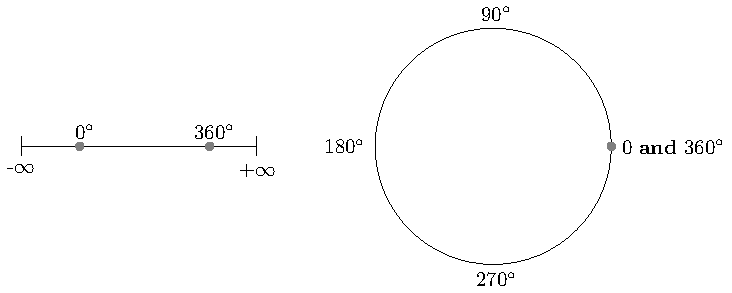
\includegraphics[width = 0.8\textwidth]{Plots/circline.pdf}
\caption{The difference between a linear scale (left) and a circular scale (right).}
\label{circline}
\end{figure}

\vspace{-0.75cm}
\section{Teacher Data}\label{Example}
\vspace{-0.75cm}
\begin{figure}
\centering
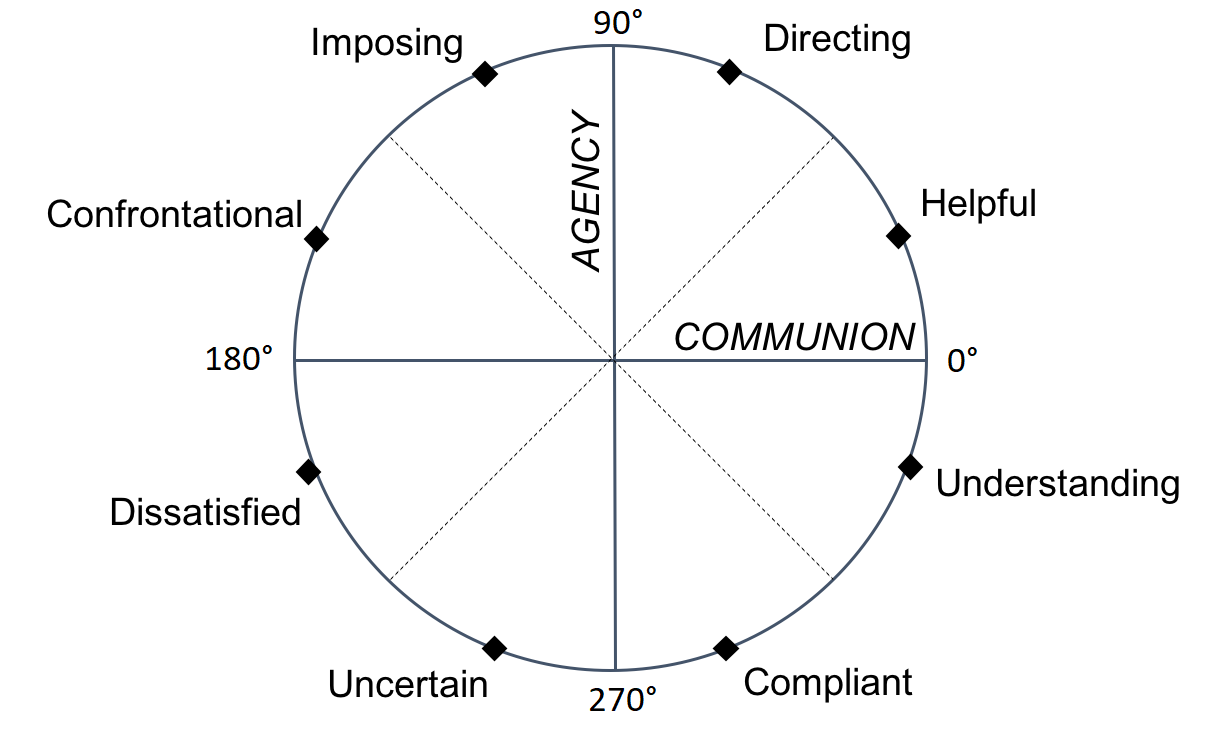
\includegraphics[width = 0.8\textwidth]{Plots/IPC-T.png}
\caption{The interpersonal circle for teachers (IPC-T). The words presented in
the circumference of the circle are anchor words to describe the type of
behavior located in each part of the IPC.}
\label{QTI}
\end{figure}

The motivating example for this article comes from the field of educational
psychology and was collected for the studies on classroom climate of
\VANDER{Want}{Van der}{van der} Want (2015), Claessens (2016) and Pennings (2017a). An
indicator of the quality of the classroom climate is the students' perception of
their teachers' interpersonal behavior. These interpersonal perceptions, both in
educational psychology as well as in other areas of psychology, can be measured
using circumplex measurement instruments (see Horowitz and Strack (2011) for an
overview of many such instruments).\newline
\indent The circumplex data used in this paper are measured using the
Questionnaire on Teacher Interaction (QTI) (Wubbels et al., 2006) which is
one such circumplex measurement instrument. The QTI is designed to measure
student perceptions of their teachers' interpersonal behavior and contains items
that load on two interpersonal dimensions: Agency and Communion. Agency refers
to the degree of power or control a teacher exerts in interaction with his/her
students. Communion refers to the degree of friendliness or affiliation a
teacher conveys in interaction with his/her students. The loadings on the two
dimensions of the QTI can be placed in a two-dimensional space formed by Agency
(vertical) and Communion (horizontal), see Figure \ref{QTI}. This space is
called the interpersonal circle/circumplex (IPC) and different parts of this
space are characterized by different teacher behavior, e.g.~\enquote{helpful} or
\enquote{uncertain}. The IPC is ``a continuous order with no beginning or end''
(Gurtman, 2009, p. 2). We call such ordering a circumplex ordering and
the IPC is therefore often called the interpersonal circumplex. The ordering
also implies that scores on the IPC could be viewed as a circular variable. This
circular variable represents the type of interpersonal behavior that a teacher
shows towards his/her students.\newline
\indent Cremers et al. (2018a) explain the circular nature of the IPC data and
analyze them as such using a circular regression model. The two dimension
scores, Agency and Communion, can be converted to a circular score using the
two-argument arctangent function in \eqref{PredVal}, where \(A\) represents a score on the Agency dimension and
\(C\) represents a score on the Communion dimension \footnote{The selection of
the origin in circumplex data depends on the scaling of the Agency and Communion
scores. Agency and Communion are measured on a scale from 1 to 5 and for
analysis purposes they are later converted to scale ranging from -1 to 1.  Their
respective 0 scores form the origin. Scaling is however only considered an issue
in those instances where cylindrical data is derived from measurements in
bivariate space.}. Note that when placing a
unit circle on Figure \ref{QTI} we see that the Agency dimension is related to
the sine of the circular score and the Communion dimension is related to the
cosine of the circular score.
\begin{equation}\label{PredVal}
\theta          = \text{atan2}\left(A, \: C\right)  =
\left\{{\begin{array}{lcl}
                                                                       \arctan\left(\frac{A}{C}\right) & \text{if}  \quad&C > 0 \\
\arctan\left(\frac{A}{C}\right) + \pi & \text{if}  \quad& C  <  0  \:\: \&\:\: A \geq 0\\
 \arctan\left(\frac{A}{C}\right) - \pi & \text{if}  \quad&C  <  0 \:\:  \&\:\:A  < 0\\
 +\frac{\pi}{2} & \text{if}  \quad& C  =  0  \:\: \&\:\:A > 0\\
 -\frac{\pi}{2} & \text{if}  \quad& C =  0  \:\: \&\:\:A < 0\\
 \text{undefined} & \text{if} \quad& C =  0   \:\: \&\:\:A = 0.
 \end{array}}
\right.
\end{equation}
The resulting circular variable \(\theta\) can then be modelled and takes values
in the interval \([0, 2\pi)\) or \([0^\circ, 360^\circ)\). Note that the round
brackets mean that \(2\pi\) and \(360^\circ\) are not included in the interval since
these represent the same value as 0 as a result of periodicity. \newline
\indent A circular analysis of circumplex data has several benefits: it is more
in line with its theoretical definition and it allows us to analyse the blend of
the two dimensions Agency and Communion instead of both dimensions separately.
This provides us with new insights compared to a separate analysis of the two
dimensions that is standard in the literature (see e.g.
Pennings et al. (2018), Wright et al. (2009) or
Wubbels et al. (2006)). There is however one main drawback: when
two-dimensional data are converted to the circle we lose some information,
namely the length of the two-dimensional vector \((A, C)^t\), \emph{i.e.}, its
Euclidean norm \(\mid\mid (A, C)^t \mid\mid\). This length represents the
strength of the interpersonal behavior a teacher shows towards his/her students.
In a cylindrical model this strength (the linear outcome) can be modeled
together with the type of interpersonal behavior of a teacher (the circular
outcome). This leads to an improved analysis of interpersonal circumplex data,
over either analyzing the two dimensions separately or using a circular model,
because we take all information, circular and linear, into account. In the next
section we introduce several cylindrical models that can be used to analyze the
teacher data. First however we will provide descriptives for the teacher data.

\vspace{-0.75cm}
\subsection{Data Description}\label{DataDescriptives}
\vspace{-0.75cm}

The teacher data was collected between 2010 and 2015 and contains several
repeated measures on the IPC of 161 teachers. Measurements were obtained using
the QTI and taken in different years and classes. For this paper we only
consider one measurement, the first occasion (2010) and largest class if data
for multiple classes were available. This results in a sample of 151 teachers.
In addition to the type of interpersonal behavior (IPC), the circular outcome,
and the strength of interpersonal behavior (IPC strength), the linear outcome, a
teachers' self-efficacy (\verb|SE|) concerning classroom management is used as
covariate in the analysis. In previous research, in psychology and education it
has been shown that higher self-efficacy is related to the quality of
interpersonal interactions (Locke \& Sadler, 2007; \VANDER{Want}{Van der}{van der} Want et al., 2018).
After listwise deletion of missings (\(3\) in total, only for the self-efficacy)
we have a sample of 148 teachers. Table \ref{Tableteacherdescriptives} shows
descriptives for the dataset. For the circular variable IPC we show sample
estimates for the circular mean \(\bar{\theta}\) and concentration \(\hat{\rho}\).
The circular concentration lies between 0, meaning the data is not concentrated
at all \emph{i.e.} spread over the entire circle, and 1, meaning all data is
concentrated at a single point on the circle. The population values of these
parameters are usually, and also in this paper, referred to as \(\mu\) (circular
location) and \(\kappa\) (circular concentration). For the linear variables
(strength IPC and SE) we show sample estimates of the linear mean and standard
deviation (sd). Figure \ref{dataplot} is a scatterplot showing the relation between
the linear and circular outcome of the teacher data for teachers with low SE
(below 1 sd below the mean), average SE (between 1 sd below and 1 sd above the
mean) and high SE (above 1 sd above the mean).

\begin{figure}
\centering
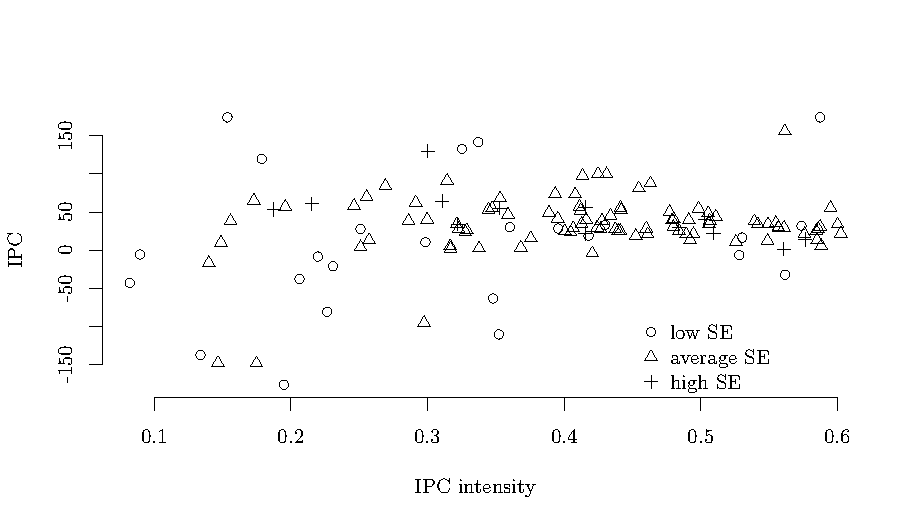
\includegraphics[width = \textwidth]{Plots/dataplot.pdf}
\caption{Plot showing the relation between the linear and circular outcome component (in degrees) of the teacher data.}
\label{dataplot}
\end{figure}

\begin{table}[h]
\centering
\caption{Descriptives for the teacher dataset.} 
\begin{tabular}{lrrrl}
  \noalign{\smallskip}\hline\noalign{\smallskip}
Variable & mean/$\bar{\theta}$ & sd/$\hat{\rho}$ & Range & Type \\ \hline\noalign{\smallskip}
IPC &33.22$^\circ$& 0.76 & - & Circular\\
strength IPC & 0.43 & 0.15 & 0.08 - 0.80 & Linear\\
SE & 5.04 & 1.00 & 1.5 - 7.0 & Linear\\
   \hline
\multicolumn{5}{l}{Note: For the circular variable IPC we show sample }\\
\multicolumn{5}{l}{estimates for the circular mean $\bar{\theta}$ and concentration $\hat{\rho}$.}\\
\multicolumn{5}{l}{For the linear variable we show the sample mean,}\\
\multicolumn{5}{l}{standard deviation and range.}
\end{tabular}
\label{Tableteacherdescriptives}
\end{table}

\vspace{-0.75cm}
\section{Four Cylindrical Regression Models}\label{Models}
\vspace{-0.75cm}

One of the goals of this paper is to show the benefits of cylindrical methods
for the analysis of circumplex data and cylindrical data in psychology in
general. To do so we decide to focus on four cylindrical models. The models were
selected for their relatively low complexity and the ease with which a
regression structure could be incorporated. But also because they show different
ways of modelling the linear and circular outcome and thereby illustrate a
wider range of cylindrical models available in the literature. The
cylindrical models contain a set of \(q\) predictors \(\boldsymbol{x} = x_1, \dots, x_q\) and \(p\) predictors \(\boldsymbol{z} = z_1, \dots, z_p\) for the linear and
circular outcomes, \(Y\) and \(\Theta\), respectively. The first two models are
based on a construction by Mastrantonio et al. (2015), while the other models are
extensions of the models from Abe and Ley (2017) and Mastrantonio (2018). The
four cylindrical models are introduced separately in the subsections below.
However, to provide a more succinct overview and comparison of the four models, Table
\ref{TableModels} gives an overview of the similarities and differences between
the models.

\begin{sidewaystable}[h]
\centering
\caption{Comparison of the four cylindrical regression models} 
\begin{tabular}{lllll}
  \noalign{\smallskip}\hline\noalign{\smallskip}
\multicolumn{1}{l}{Aspect} & CL-PN & CL-GPN  & Abe-Ley  & GPN-SSN \\ \hline\noalign{\smallskip}
$\Theta$ & &&&\\
$\:\:$Distribution& PN & GPN & Sine-skewed vM & GPN\\
$\:\:$Domain & $[0, 2\pi)$ & $[0, 2\pi)$ & $[0, 2\pi)$ & $[0, 2\pi)$\\
$\:\:$Shape & symmetric, & asymmetric, & asymmetric, & asymmetric, \\
            & unimodal  & multimodal & unimodal   & multimodal \\\hline\noalign{\smallskip}
$Y$& &&&\\
$\:\:$Distribution & Normal & Normal & Weibull & skewed-Normal\\
$\:\:$Domain & $(-\infty, + \infty)$ & $(-\infty, + \infty)$ & $(0, + \infty)$ & $(-\infty, + \infty)$\\
$\:\:$Shape & symmetric, & symmetric, & asymmetric, & asymmetric, \\
            & unimodal  & unimodal  & unimodal   & unimodal\\\hline\noalign{\smallskip}
$\Theta$-$Y$ dependence &                                   &                                   & & \\
                        & $y$ regressed on                  & $y$ regressed on                  & $\alpha$ and $\kappa$ & multivariate \\
                        & $\sin(\theta)$ and $\cos(\theta)$ & $\sin(\theta)$ and $\cos(\theta)$ & & distribution\\\hline
\multicolumn{5}{l}{Note: PN and GPN refer to the projected normal and general projected normal distribution.}\\
\multicolumn{5}{l}{vM refers to the von-Mises distribution}\\

\end{tabular}
\label{TableModels}
\end{sidewaystable}

\vspace{-0.75cm}
\subsection{The Modified Circular-Linear Projected Normal (CL-PN) and Modified Circular-Linear General Projected Normal (CL-GPN) Models}\label{CL-(G)PN}
\vspace{-0.75cm}

Following Mastrantonio et al. (2015) we consider two models where
the relation between \(\Theta \in [0, 2\pi)\) and \(Y\in (-\infty, + \infty)\)
and \(q\) covariates is specified as
\begin{equation}\label{circlinlink}
Y = \gamma_0 + \gamma_{cos}*\cos(\Theta)*R + \gamma_{sin}*\sin(\Theta)*R + \gamma_1*x_1 + \dots + \gamma_q*x_q +  \epsilon,
\end{equation}
\noindent where the random variable \(R\geq0\) will be introduced below, the
error term \(\epsilon \sim N(0, \sigma^2)\) with variance \(\sigma^2>0\),
\(\gamma_0, \gamma_{cos}, \gamma_{sin}, \gamma_1, \dots, \gamma_q\) are the
intercept and regression coefficients and \(x_1, \dots, x_q\) are the \(q\)
covariates for the prediction of the linear outcome. We thus assume a normal
distribution for the linear outcome.\newline
\indent For the circular outcome we assume either a projected normal (PN) or a
general projected normal (GPN) distribution. These distributions arise from a
projection of a distribution defined in bivariate space onto the circle. Figure
\ref{projection} represents this projection. In the left plot of Figure
\ref{projection} we see datapoints from the bivariate variable
\(\boldsymbol{S}\) that in the middle plot are projected to form the circular
outcome \(\Theta\) in the right plot. Mathematically the relation between
\(\boldsymbol{S}\) and \(\Theta\) is defined as follows
\begin{equation}\label{projection}
\boldsymbol{S} = \begin{bmatrix} S^{I} \\ S^{II} \end{bmatrix} = R\boldsymbol{u} = \begin{bmatrix} R \cos (\Theta) \\  R\sin (\Theta) \end{bmatrix},
\end{equation}
\noindent where \(R = \mid\mid \boldsymbol{S} \mid\mid\), the Euclidean norm of
\(\boldsymbol{S}\); the lines connecting the bivariate datapoints to the origin
in the middle plot. We call \(\boldsymbol{S}\) the augmented representation of the
circular outcome. It is a variable that in contrast to \(\Theta\) is not
observed and thus considered latent or auxiliary. This then means that we do not
model \(\Theta\) directly but indirectly through \(\boldsymbol{S}\). \newline
\indent For both the PN and GPN distributions the circular location parameter
\(\mu\in [0, 2\pi)\) is modeled as \(\hat{\mu}_i = \mbox{atan2}(\hat{\mu}_i^{II}, \hat{\mu}_i^{I}) = \mbox{atan2}(\boldsymbol{\beta}^{II}\boldsymbol{z}_i, \boldsymbol{\beta}^{I}\boldsymbol{z}_i)\)\footnote{Note that for the CL-GPN
model the circular location parameter also depends on the variance-covariance
matrix and the circular predicted values should be computed using numerical
integration or Monte Carlo methods because a closed form expression for the mean
direction is not available.} where \(\boldsymbol{\beta}^{I}\) and
\(\boldsymbol{\beta}^{II}\) are vectors with intercepts and regression
coefficients for the prediction of \(\boldsymbol{S}\) and \(\boldsymbol{z}_i\) is a
vector with predictor values for each individual \(i \in 1, \dots, n\) where \(n\)
is the sample size. Note that as a result of the augmented representation of the
circular outcome we have two sets of regression coefficients and intercepts, one
for each bivariate component of \(\boldsymbol{S}\). This leads to problems when we
want to interpret the effect of a covariate on the circle. A circular regression
line is shown in Figure \ref{circregline}, with covariate values on the x-axis
and the predicted circular outcome on the y-axis. As can be seen it is of a
non-linear character meaning that the effect of a covariate is different at
different values of the covariate. A circular regression line is usually
described by the slope at the inflection point, the point at which the slope of
the regression line starts flattening off (indicated with a square in Figure
\ref{circregline}). By default, the parameters from the PN and GPN models do not
directly describe this inflection point. For the PN distribution however,
Cremers et al. (2018b) solved this interpretation problem and introduce new
circular regression coefficients. They introduce a new parameter \(b_c\) that
describes the slope at the inflection point of the regression line. For the
GPN distrbution the interpretation problem however remains.\newline
\indent The main difference between the PN and GPN distribution lies in the
definition of their covariance matrix. For the PN distribution this is an
identity matrix, causing the distribution to be unimodal and symmetric, whereas
for the GPN distribution \(\boldsymbol{\Sigma} = \begin{bmatrix} \tau^2 + \xi^2 & \xi\\ \xi & 1 \end{bmatrix}\) where \(\xi,\tau \in (-\infty, +\infty)\), allowing for multimodality and
asymmetry/skewness.\newline
\indent For the teacher dataset the predicted linear outcome, strengths of
interpersonal behavior, in the CL-PN and CL-GPN model is the following:
\[\hat{y}_i = \gamma_0 + \gamma_{cos}\cos(\theta_i)r_i +
\gamma_{sin}\sin(\theta_i)r_i + \gamma_1\text{SE}_i.\] The predicted circular
outcome, type of interpersonal behavior, equals: \[\hat{\theta}_i = \mu_i =
\mbox{atan2} (\beta_0^{II} + \beta_1^{II}\text{SE}_i, \beta_0^{I} +
\beta_1^{I}\text{SE}_i).\] \noindent where \(\text{SE}_i\) is the self-efficacy
score of one individual. The CL-PN and CL-GPN models thus allow us to assess the
average type and strength of interpersonal behavior through the parameters
\(\beta_{0}^{I}\), \(\beta_{0}^{II}\) and \(\gamma_0\) as well as the effect of
self-efficacy on type and strength of teacher behavior through the parameters,
\(\beta_{1}^{I}\), \(\beta_{1}^{II}\) and \(\gamma_1\). In addition, because the type
and strength of interpersonal behavior are modelled together via the regression
in \eqref{circlinlink} we can assess the effect of the type of interpersonal
behavior on the strength through the parameters \(\gamma_{sin}\) and
\(\gamma_{cos}\). In the teacher data these are the regression coefficients for
the effect of the sine and cosine of the type of behavior which are related to
the scores on the Agency and Communion dimensions respectively.\newline
\indent Both the CL-PN and CL-GPN models are estimated using Markov Chain Monte
Carlo (MCMC) methods based on Nuñez-Antonio, Gutiérrez-Peña, and Escarela (2011), Wang and Gelfand (2013) and
Hernandez-Stumpfhauser, Breidt, and Woerd (2016) for the regression of the circular outcome. A detailed
description of the Bayesian estimation and MCMC samplers can be found in the
Supplementary Material.

\begin{figure}
\centering
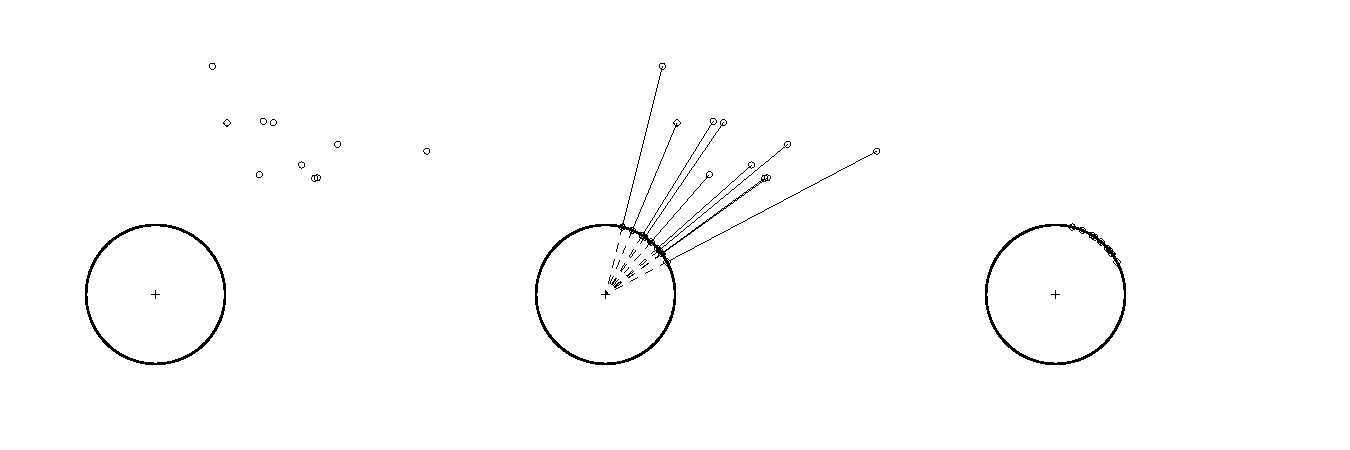
\includegraphics[width = \textwidth]{Plots/plotprojecting.pdf}
\caption{Plot showing the projection of datapoints in bivariate space, $\boldsymbol{S}$, (left) to the circle (right). The lines connecting the bivariate datapoints to the circular datapoints represent the euclidean norm of the bivariate datapoints, the random variable $R$.}
\label{projection}
\end{figure}

\begin{figure}[]
  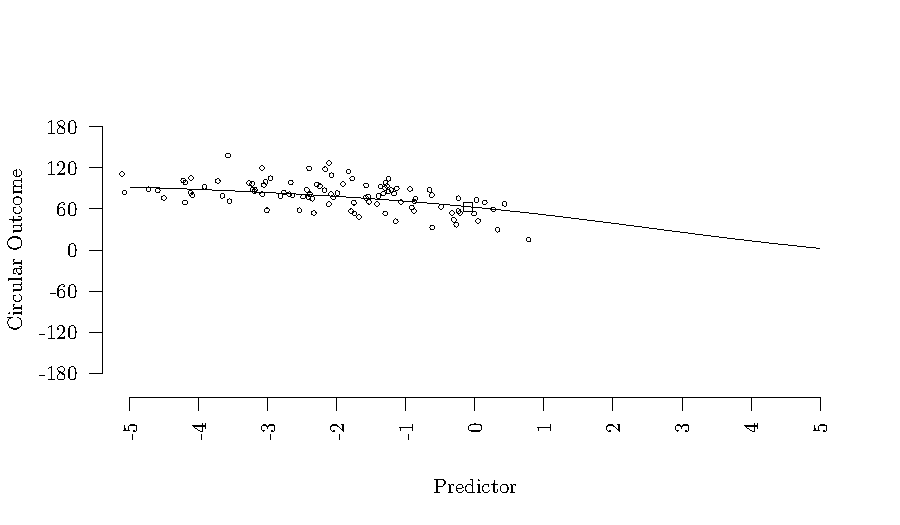
\includegraphics[width = \textwidth]{Plots/circregline.pdf}
  \caption{Circular regression line for the relation between a covariate and a circular outcome with the data the regression line was fit to. The square indicates the inflection point of the regression line.}
  \label{circregline}
\end{figure}

\vspace{-0.75cm}
\subsection{The Modified Abe-Ley Model}\label{WeiSSVM}
\vspace{-0.75cm}

This model is an extension of the cylindrical model introduced in
Abe and Ley (2017) to the regression context. It concerns a combination
of a Weibull distribution, with scale parameter \(\nu>0\) and shape parameter
\(\alpha\), for the linear outcome and a sine-skewed von Mises distribution,
with location parameter \(\mu\in [0, 2\pi)\), concentration parameter
\(\kappa>0\) and skewness \(\lambda \in [-1,1]\), for the circular outcome. In
contrast to the CL-PN and CL-GPN models, the linear outcome \(Y\) is in this
model defined only on the positive real half-line \([0, + \infty)\) and thus can
not be negative.\newline
\indent In this model we predict the linear scale parameter and circular
location parameter, both of which we can express in terms of
covariates: \(\hat{\nu}_i = \exp(\boldsymbol{x}_i^t\boldsymbol{\gamma}) > 0\) and
\(\hat{\mu}_i = \beta_0 + 2\tan^{-1}(\boldsymbol{z}_i^t\boldsymbol{\beta})\). The
parameter \(\boldsymbol{\gamma}\) is a vector of \(q\) regression coefficients
\(\gamma_j \in (-\infty, +\infty)\) for the prediction of \(y\) where \(j = 0, \dots, q\) and \(\gamma_0\) is the intercept. The parameter \(\beta_0 \in [0, 2\pi)\) is the intercept and \(\boldsymbol{\beta}\) is a vector of \(p\)
regression coefficients \(\beta_j \in (-\infty, +\infty)\) for the prediction of
\(\theta\) where \(j = 1, \dots, p\). The vector \(\boldsymbol{x}_i\) is a
vector of predictor values for the prediction of \(y\) and \(\boldsymbol{z}_i\)
is a vector of predictor values for the prediction of \(\theta\).\newline
\indent For the teacher data, the predicted values for the circular outcome in
the Abe-Ley model are: \[\hat{\theta}_{i} = \hat{\mu}_i = \beta_0 + 2 *
\tan^{-1}(\beta_1\text{SE}_i).\] We do not directly predict the linear outcome.
The conditional distribution for the linear outcome is Weibull, meaning that we
can use methods from survival analsis to interpret the effect of a predictor. In
survival analysis a \enquote{survival} function is used in which time is plotted against
the probability of survival of subjects suffering from a specific medical
condition. In the teacher data we can thus compute the probability of a teacher
having a specific strength on the IPC. This probability is computed using the
\enquote{survival-function} defined as \[\exp(-\alpha
y_i^{\hat{\nu}_i(1-\tanh(\kappa)\cos(\theta_i - \hat{\mu}_i))^{1/\alpha}}),\]
with \(\hat{\nu}_i = \exp(\gamma_0 + \gamma_1\mbox{SE}_i)\). From the survival
function we also see that the circular concentration parameter \(\kappa\) and
the linear shape parameter \(\alpha\) regulate the circular-linear dependence in
the Abe-Ley model. The Abe-Ley model thus allows us to assess the average type
and strength of interpersonal behavior through the parameters \(\beta_{0}\) and
\(\gamma_0\) as well as the effect of self-efficacy on type and strength of
teacher behavior through the parameters \(\beta_{1}\) and \(\gamma_1\).\newline
\indent We can use numerical optimization (Nelder-Mead) to find solutions for
the maximum likelihood (ML) estimates for the parameters of the model.

\vspace{-0.75cm}
\subsection{Modified Joint Projected and Skew Normal Model (GPN-SSN)}\label{CL-GPN_multivariate}
\vspace{-0.75cm}

This model is an extension of the cylindrical model introduced by
Mastrantonio (2018) to the regression context. The model contains \(m\)
independent circular outcomes and \(w\) independent linear outcomes. The
circular outcomes \(\boldsymbol{\Theta} = (\boldsymbol{\Theta}_1, \dots,  \boldsymbol{\Theta}_m)\) are modelled together by a multivariate GPN
distribution. The linear outcomes \(\boldsymbol{Y} = (\boldsymbol{Y}_1, \dots,  \boldsymbol{Y}_w)\) are modelled together by a multivariate skew normal
distribution (Sahu, Dey, \& Branco, 2003). Because the GPN distribution is modelled
using a so-called augmented representation (see also the description of the
CL-PN and CL-GPN models) it is convenient to use a similar tactic for
modelling the multivariate skew normal distribution. As in
Mastrantonio (2018), dependence between the linear and circular outcome is
created by modelling the augmented representations of \(\boldsymbol{\Theta}\)
and \(\boldsymbol{Y}\) together in a \(2m + w\) dimensional normal
distribution.\newline
\indent This means that we have a shared mean vector and variance-covariance
matrix for the linear and circular outcome(s), much like having multiple
outcomes in a MANOVA (multivariate analysis of variance) model. In our
regression extension of the GPN-SSN model we have \(i = 1, \dots, n\)
observations of \(m\) circular outcomes, \(w\) linear outcomes and \(g\)
covariates. The mean vector then becomes \(\boldsymbol{M}_i = \boldsymbol{B}^t\boldsymbol{x}_i\) where \(\boldsymbol{B}\) is a \((g + 1) \times (2m + w)\) matrix with regression coefficients and intercepts and
\(\boldsymbol{x}_i\) is a \(g + 1\) dimensional vector containing the value 1 to
estimate an intercept and the \(g\) covariate values. This means that in contrast
to the other three models, we have to use the same set of predictors for the
circular and linear outcome.\newline
\indent For the teacher data, \(\boldsymbol{B} = \begin{bmatrix} \beta_{0_{s^{I}}} & \beta_{0_{s^{II}}} & \beta_{0_{y}}\\ \beta_{1_{s^{I}}} & \beta_{1_{s^{II}}} & \beta_{1_{y}} \end{bmatrix}\). The predicted circular\footnote{Note that for the  GPN-SSN model the predicted circular outcome also depends on the variance-covariance matrix and the circular predicted values should be computed using numerical integration or Monte Carlo methods because a closed form expression for the mean direction is not available.} and
linear outcomes in the GPN-SSN model are
\[\hat{\theta_i} = \mbox{atan2}(\beta_{0_{s^{II}}} +
\beta_{1_{s^{II}}}\text{SE}_i,\beta_{0_{s^{I}}} +
\beta_{1_{s^{I}}}\text{SE}_i),\]

\noindent and

\[\hat{y_i} = \beta_{0_{y_i}} +
\beta_{1_{y_i}}\text{SE}_i.\]

\noindent The GPN-SSN model thus allows us to assess the average type and
strength of interpersonal behavior through the parameters \(\beta_{0_{s^{I}}}\),
\(\beta_{0_{s^{II}}}\) and \(\beta_{0_{y}}\) as well as the effect of self-efficacy
on type and strength of teacher behavior through the parameters
\(\beta_{1_{s^{I}}}\), \(\beta_{1_{s^{II}}}\) and \(\beta_{1_{y}}\). In addition,
because the type and strength of interpersonal behavior are modelled together
using a multivariate normal distribution we can, through its variance-covariance
matrix, also assess the dependence between the type and strength of interpersonal
behavior. \newpage
\indent We estimate the model using MCMC methods. A detailed description of these
methods is given in the Supplementary Material.

\vspace{-0.75cm}
\subsection{Model Fit Criterion}\label{Modelfit}
\vspace{-0.75cm}

For the four cylindrical models we focus on their out-of-sample predictive
performance to determine the fit of the model. To do so we use k-fold
cross-validation and split our data into 10 folds. Each of these folds (10 \(\%\)
of the sample) is used once as a holdout set and 9 times as part of a training
set. The analysis will thus be performed 10 times, each time on a different
training set.\newline
\indent A proper criterion to compare out-of-sample predictive performance is
the Predictive Log Scoring Loss (PLSL) (Gneiting \& Raftery, 2007). The lower the
value of this criterion, the better the predictive performance of the model.
Using ML estimates this criterion can be computed as follows:
\begin{equation}\label{PLSLML}
PLSL = -2 \sum_{i = 1}^{M}\log l(x_i \mid \hat{\boldsymbol{\vartheta}}),\nonumber
\end{equation}
\noindent where \(l\) is the model likelihood, \(M\) is the sample size of the
holdout set, \(x_i\) is the \(i^{th}\) datapoint from the holdout set and
\(\hat{\boldsymbol{\vartheta}}\) are the ML estimates of the model parameters.
Using posterior samples the criterion is similar to the log pointwise predictive
density (lppd) (Gelman et al., 2014, p. 169) and can be computed as:
\begin{equation}\label{PLSLBayes}
PLSL = -2 \frac{1}{B} \sum_{j = 1}^{B}\sum_{i = 1}^{M} \log l(x_i \mid \boldsymbol{\vartheta}^{(j)}),\nonumber
\end{equation}
\noindent where \(B\) is the amount of posterior samples and
\(\boldsymbol{\vartheta}^{(j)}\) are the posterior estimates of the model
parameters for the \(j^{th}\) iteration. Because the joint density and thus also
the likelihood for the modified GPN-SSN model is not
available in closed form (Mastrantonio, 2018) we compute the PLSL for the
circular and linear outcome separately for all models. Note that although we fit
the CL-PN, CL-GPN and GPN-SSN models using Bayesian statistics, we do not take
prior information into account when assessing model fit with the PLSL. According
to Gelman et al. (2014) this is not necessary since we are assessing the fit of a model
to data, the holdout set, only. They argue that the prior in such case is only
of interest for estimating the parameters of the model but not for determining
the predictive accuracy.\newline
\indent For each of the four cylindrical models and for each of the 10
cross-validation analyses we can then compute a PLSL for the circular and linear
outcome by using the conditional log-likelihoods of the respective outcome (see
Supplementary Material for a definition of the loglikelihoods). To evaluate the
predictive performance we average across the PLSL criteria of the
cross-validation analyses. We also assess the cross-validation variability by
means of the standard deviations of the PLSL criteria.

\vspace{-0.75cm}
\section{Results}\label{DataAnalysis}
\vspace{-0.75cm}

In this section we analyze the teacher data with the help of the four
cylindrical models from the previous section. We will present the results,
posterior estimates and their interpretation for all four models.

\vspace{-0.75cm}
\subsection{Analysis}\label{DataResults}
\vspace{-0.75cm}

In the Supplementary Material we have described the starting values for the MCMC
procedures for the CL-PN, CL-GPN and GPN-SSN models, hence it remains to specify
the starting values for the maximum likelihood based Abe-Ley model: \(\eta_0 = 0.9, \eta_1 = 0.9, \nu_0 = 0.9, \nu_1 = 0.9, \kappa = 0.9, \alpha = 0.9, \lambda = 0\). The initial number of iterations for the three MCMC samplers was set to
2000. After convergence checks via traceplots we concluded that some of the
parameters of the GPN-SSN model did not converge. Therefore we set the number of
iterations of the MCMC models to 20,000 and subtracted a burn-in of 5000 to
reach convergence (the Geweke diagnostics show absolute z-scores over 1.96 in
6\% of the estimated parameters). Note that we choose the same number of
iterations for all three models estimated using MCMC procedures to make
their comparison via the PLSL as fair as possible. Lastly, the predictor
\verb|SE| was centered before inclusion in the analysis as this allows the
intercepts to bear the classical meaning of average behavior.\newline
\indent Tables \ref{tab:estCLGPN}, \ref{tab:estAL} and \ref{tab:estCLGPNM} show
the results for the four cylindrical models that were fit to the teacher data.
For the models estimated using MCMC methods, CL-PN, CL-GPN and GPN-SSN, we show
descriptives of the posterior of the estimated parameters (posterior mode and
lower and upper bound of the 95\% highest posterior density (HPD) interval). For
the Abe-Ley model we show the maximum likelihood estimates of the parameters. To
compare the results of the four models we focus on the following aspects: the
estimated average scores (intercept) on the type and strength of interpersonal
behavior (1), the effect of self-efficacy on the type and strength of
interpersonal behavior (2), the dependence between the type and strength of
interpersonal behavior (3) and the model fit (4).

\begin{table}

\caption{\label{tab:estCLGPN}Results, cross-validation mean and standard deviation, for the modified CL-PN and CL-GPN models}
\centering
\begin{tabular}[t]{lllllll}
\toprule
\multicolumn{1}{c}{Parameter} & \multicolumn{3}{c}{CL-PN} & \multicolumn{3}{c}{CL-GPN} \\
\cmidrule(l{2pt}r{2pt}){1-1} \cmidrule(l{2pt}r{2pt}){2-4} \cmidrule(l{2pt}r{2pt}){5-7}
  & Mode & HPD LB & HPD UB & Mode & HPD LB & HPD UB\\
\midrule
$\beta_0^{I}$ & 1.76 (0.09) & 1.50 (0.07) & 2.03 (0.09) & 2.43 (0.12) & 1.91 (0.10) & 3.05 (0.17)\\
$\beta_1^{I}$ & 0.65 (0.07) & 0.42 (0.06) & 0.90 (0.08) & 0.84 (0.11) & 0.45 (0.09) & 1.29 (0.15)\\
$\beta_0^{II}$ & 1.15 (0.05) & 0.92 (0.04) & 1.37 (0.04) & 1.47 (0.05) & 1.16 (0.04) & 1.78 (0.05)\\
$\beta_1^{II}$ & 0.58 (0.03) & 0.38 (0.04) & 0.79 (0.04) & 0.70 (0.06) & 0.47 (0.05) & 0.96 (0.08)\\
$\gamma_0$ & 0.38 (0.01) & 0.31 (0.01) & 0.44 (0.01) & 0.37 (0.01) & 0.31 (0.01) & 0.42 (0.01)\\
\addlinespace
$\gamma_{cos}$ & 0.04 (0.00) & 0.01 (0.00) & 0.06 (0.00) & 0.03 (0.00) & 0.01 (0.00) & 0.04 (0.00)\\
$\gamma_{sin}$ & -0.01 (0.00) & -0.04 (0.00) & 0.02 (0.00) & -0.00 (0.00) & -0.03 (0.00) & 0.03 (0.00)\\
$\gamma_1$ & 0.03 (0.01) & -0.00 (0.00) & 0.07 (0.01) & 0.03 (0.00) & -0.00 (0.00) & 0.06 (0.00)\\
$\sigma$ & 0.14 (0.00) & 0.12 (0.00) & 0.16 (0.00) & 0.14 (0.00) & 0.12 (0.00) & 0.16 (0.00)\\
$\sum_{1,1}$ & NA (NA) & NA (NA) & NA (NA) & 3.04 (0.29) & 1.85 (0.13) & 5.00 (0.41)\\
\addlinespace
$\sum_{1,2}$ & NA (NA) & NA (NA) & NA (NA) & 0.47 (0.12) & 0.12 (0.12) & 0.80 (0.10)\\
$\sum_{2,2}$ & NA (NA) & NA (NA) & NA (NA) & 1.00 (0.00) & 1.00 (0.00) & 1.00 (0.00)\\
\bottomrule
\multicolumn{7}{l}{Note: $\beta_0^{I}$, $\beta_0^{II}$ and $\gamma_0$ inform us about the type and strength of interpersonal behavior}\\
\multicolumn{7}{l}{at the average self-efficacy. $\beta_1^{I}$, $\beta_1^{II}$ and $\gamma_1$ inform us about the effect of self-efficacy on the}\\
\multicolumn{7}{l}{type and strength of interpersonal behavior. $\gamma_{cos}$ and $\gamma_{sin}$ inform us about the dependence}\\
\multicolumn{7}{l}{ between the type and strength of interpersonal behavior. $\sum_{1,1}$, $\sum_{1,2}$ and $\sum_{2,2}$ are}\\
\multicolumn{7}{l}{elements of the variance-covariance matrix of the type of interpersonal behavior in the}\\
\multicolumn{7}{l}{CL-GPN model and $\sigma$ is the error standard deviation of the strength of interpersonal behavior.}\\

\end{tabular}
\end{table}

\begin{table}

\caption{\label{tab:estAL}Results, cross-validation mean and standard deviation (SD), for the modified Abe-Ley model}
\centering
\begin{tabular}[t]{llllllll}
\toprule
& $\beta_0$ & $\beta_1$ & $\gamma_0$  & $\gamma_1$ & $\alpha$ & $\kappa$ & $\lambda$\\
Mean & 0.36 & -0.03 & 1.17 & 0.04 & 3.66 & 1.51 & 0.70 \\
SD & 0.02 & 0.01 & 0.02 & 0.02 & 0.12 & 0.08 & 0.05\\
\bottomrule
\multicolumn{8}{l}{Note: $\beta_0$  and $\gamma_0$ inform us about the type and strength }\\
\multicolumn{8}{l}{of interpersonal behavior at the average self-efficacy. $\beta_1$ }\\
\multicolumn{8}{l}{and $\gamma_1$ inform us about the effect of self-efficacy on the}\\
\multicolumn{8}{l}{type and strength of interpersonal behavior. $\alpha$ is the } \\
\multicolumn{8}{l}{shape parameter of the distribution of the strength }\\
\multicolumn{8}{l}{of interpersonal bahavior. $\kappa$ and $\lambda$ are the concentration}\\
\multicolumn{8}{l}{and skewness parameters for the distribution of the type}\\
\multicolumn{8}{l}{of interpersonal behavior.}\\
\end{tabular}
\end{table}

\begin{table}
\caption{\label{tab:estCLGPNM}Results, cross-validation mean and standard deviation, for the GPN-SSN model}
\centering
\begin{tabular}[t]{lllllll}
\toprule
\multicolumn{1}{c}{Parameter} & \multicolumn{3}{c}{Unconstrained} & \multicolumn{3}{c}{Constrained} \\
\cmidrule(l{2pt}r{2pt}){1-1} \cmidrule(l{2pt}r{2pt}){2-4} \cmidrule(l{2pt}r{2pt}){5-7}
  & Mode & HPD LB & HPD UB & Mode & HPD LB & HPD UB\\
\midrule
$\beta_{0_s^{I}}$ & 0.30 (0.01) & 0.26 (0.01) & 0.34 (0.01) & 2.11 (0.11) & 1.75 (0.09) & 2.50 (0.11)\\
$\beta_{0_s^{II}}$ & 0.19 (0.00) & 0.17 (0.01) & 0.21 (0.00) & 1.34 (0.06) & 1.10 (0.05) & 1.57 (0.06)\\
$\beta_{0_y}$ & 0.33 (0.01) & 0.30 (0.30) & 0.36 (0.01) & 0.33 (0.01) & 0.30 (0.01) & 0.36 (0.01)\\
\addlinespace
$\beta_{1_s^{I}}$ & 0.09 (0.01) & 0.05 (0.01) & 0.13 (0.01) & 0.60 (0.06) & 0.33 (0.05) & 0.90 (0.06)\\
$\beta_{1_s^{II}}$ & 0.07 (0.00) & 0.04 (0.00) & 0.09 (0.01) & 0.48 (0.03) & 0.30 (0.04) & 0.66 (0.04)\\
$\beta_{1_y}$ & 0.09 (0.01) & 0.06 (0.06) & 0.12 (0.01) & 0.09 (0.01) & 0.06 (0.01) & 0.12 (0.01)\\
\addlinespace
$\sum_{s_{1,1}}$ & 0.05 (0.00) & 0.04 (0.00) & 0.06 (0.00) & 2.44 (0.15) & 1.72 (0.07) & 3.46 (0.14)\\
$\sum_{s_{2,2}}$ & 0.02 (0.00) & 0.02 (0.00) & 0.03 (0.00) & 1.00 (0.00) & 1.00 (0.00) & 1.00 (0.00)\\
$\sum_{y_{3,3}}$ & 0.03 (0.00) & 0.02 (0.02) & 0.04 (0.00) & 0.03 (0.00) & 0.02 (0.00) & 0.04 (0.00)\\
$\sum_{s_{1,2}}$ & 0.00 (0.00) & -0.00 (0.00) & 0.01 (0.00) & 0.08 (0.06) & -0.20 (0.06) & 0.34 (0.06)\\
$\sum_{sy_{1,3}}$ & 0.03 (0.00) & 0.02 (0.00) & 0.04 (0.00) & 0.23 (0.01) & 0.17 (0.00) & 0.32 (0.01)\\
$\sum_{sy_{2,3}}$ & 0.01 (0.00) & 0.01 (0.01) & 0.02 (0.00) & 0.09 (0.01) & 0.06 (0.01) & 0.12 (0.01)\\
$\lambda$ & 0.16 (0.01) & 0.14 (0.01) & 0.18 (0.01) & 0.16 (0.01) & 0.14 (0.01) & 0.18 (0.01)\\
\bottomrule
\multicolumn{7}{l}{Note: $\beta_{0_s^{I}}$, $\beta_{0_s^{II}}$ and $\beta_{0_y}$ inform us about the type and strength of interpersonal behavior}\\
\multicolumn{7}{l}{at the average self-efficacy. $\beta_{1_s^{I}}$, $\beta_{1_s^{II}}$ and $\beta_{1_y}$ inform us about the effect of self-efficacy }\\
\multicolumn{7}{l}{on the type and strength of interpersonal behavior. $\sum_{s_{1,1}}$, $\sum_{s_{1,2}}$, $\sum_{s_{2,2}}$, $\sum_{y_{3,3}}$, $\sum_{sy_{1,3}}$,  and $\sum_{sy_{2,3}}$ }\\
\multicolumn{7}{l}{are elements of the variance-covariance matrix of which $\sum_{sy_{1,3}}$ and $\sum_{sy_{2,3}}$ inform us about}\\
\multicolumn{7}{l}{the dependence between the type and strength of interpersonal behavior.}\\
\multicolumn{7}{l}{$\lambda$ is the skewness parameter of the distribution of the strengths of interpersonal behavior.}\\
\end{tabular}
\end{table}

\vspace{-0.5cm}
\subsubsection{Average type and strength of interpersonal behavior}

The parameters \(\gamma_0\) in the CL-PN, CL-GPN and Abe-Ley model and the
parameter \(\beta_{0_y}\) in the GPN-SSN model inform us about the strength of
interpersonal behavior at the average self-efficacy. For the CL-PN, CL-GPN and
GPN-SSN models the parameters are estimated at 0.38, 0.37 and 0.33 respectively
and are a direct prediction of the strength of interpersonal behavior at the
average self-efficacy. The estimate for the GPN-SSN model is notably lower and
likely to be caused by its skewed distribution for the strengths of
interpersonal behavior. In the Abe-Ley model, \(\gamma_0\) influences the shape
parameter of the distribution of the strength of interpersonal behavior and does
not directly estimate the average strength. Instead we can use the survival
function to say something about the probability of having a certain strength of
interpersonal behavior. Figure \ref{reglineweib} shows this function for several
values of self-efficacy. We look at the survival function at average values of
self-efficacy. Note that this function is the average of all survival functions
for observations that fall within 1 standard deviation of the mean. The survival
function indicates that the probability of having a low strength of
interpersonal behavior is higher than having a high strength. We however can not
make any direct statement about the estimated strength using the Abe-Ley
model.\newline
\indent The parameters \(\beta_0^{I}\), \(\beta_0^{II}\), \(\beta_0\),
\(\beta_{0_{s^{I}}}\) and \(\beta_{0_{s^{II}}}\) inform us about the type of
interpersonal behavior at the average self-efficacy for the CL-PN, CL-GPN,
Abe-Ley and GPN-SSN model respectively. For the CL-PN, CL-GPN and GPN-SSN model
we need to combine the estimates for the underlying bivariate components \(\{I, II\}\) into one circular estimate using the double arctangent
function\footnote{\(\mbox{atan2}(\beta_0^{II}, \beta_0^{I})\) or
\(\mbox{atan2}(\beta_{0_{s^{II}}}, \beta_{0_{s^{I}}})\)}.
Table \ref{tab:means} shows that these circular estimates are similar for the
three models at 32.29\(^\circ\), 33.70\(^\circ\) and 35.53\(^\circ\). In the Abe-Ley
model the type of interpersonal behavior at the average self-efficacy is
estimated at 0.36 radians or 20.63\(^\circ\).

\begin{figure}
\centering
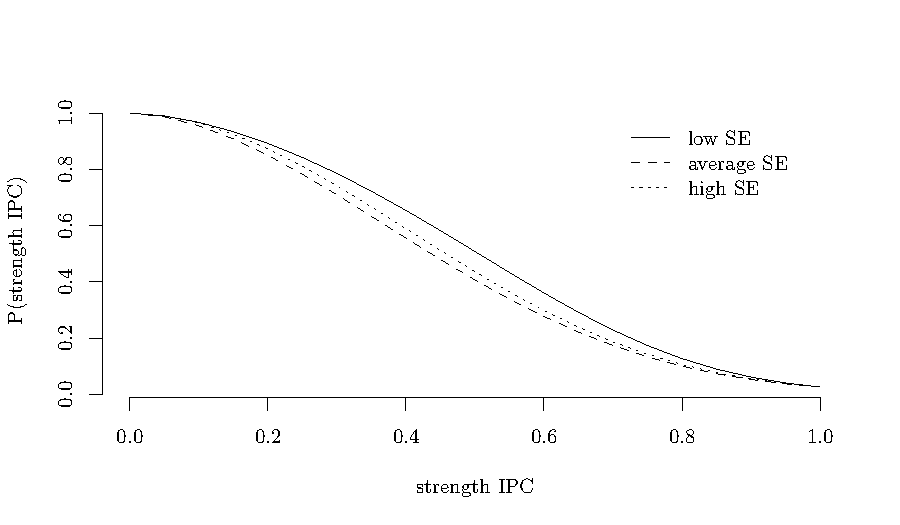
\includegraphics[width = \textwidth]{Plots/survivaldiffSE.pdf}
\caption{Plot showing the probability of having a particular strength of interpersonal behavior (survival plot) for the minimum, mean and maximum self-efficacy in the data.}
\label{reglineweib}
\end{figure}

\begin{table}
\caption{\label{tab:means}Posterior estimates (in degrees) for the circular mean (at SE = 0) in the CL-PN, CL-GPN and GPN-SSN models}
\centering
\begin{tabular}[t]{lrrr}
\toprule
  & Mode & HPD LB & HPD UB\\
  \midrule
CL-PN & 32.29 & 24.81 & 39.71\\
CL-GPN & 33.70 & 26.72 & 41.15\\
GPN-SSN & 35.53 & 28.40 & 43.30\\
\bottomrule
\multicolumn{4}{l}{Note that these means are based on}\\
\multicolumn{4}{l}{their posterior predictive distribution }\\
\multicolumn{4}{l}{following (Wang and Gelfand, 2013)}\\
\end{tabular}
\end{table}

\vspace{-0.5cm}
\subsubsection{The effect of self-efficacy}

The parameters \(\gamma_1\) in the CL-PN, CL-GPN, Abe-Ley models and \(\beta_{1_y}\)
in the GPN-SSN model inform us about the effect of self-efficacy on the strength
of interpersonal behavior. For the CL-PN, CL-GPN and GPN-SSN model the
parameters are estimated at 0.03, 0.03 and 0.09 respectively and are a direct
estimate of the effect of self-efficacy on the strength of interpersonal
behavior, \emph{i.e.} an increase of 1 unit in self-efficacy leads to an
increase of 0.09 units in the strength of interpersonal behavior according to
the GPN-SSN model. These estimates are however quite small and only different
from 0 (the HPD interval does not contain 0) in the GPN-SSN model. It is hard to
say which of the three models, CL-PN, CL-GPN or GPN-SSN, to use to base our
conclusions on. The models CL-GPN and CL-PN fit the linear outcome best according
to the model fit in Table \ref{tab:ModelFit}. In these models the linear outcome has a
symmetric distribution whereas in the GPN-SSN the distribution of the linear
outcome is skewed. However, the effect of self-efficacy is different from 0 only
in the GPN-SSN model which does not seem to match with its lower model fit.\newline
\indent In the Abe-Ley model, \(\gamma_1\) influences the shape parameter of the distribution of
the strength of interpersonal behavior and does not directly estimate the effect
of self-efficacy. Instead we can use the survival function to say something
about the probability of having a certain strength of interpersonal behavior for
different values of self-efficacy. Figure \ref{reglineweib} shows this function
for low, average and high values of self-efficacy (as defined in Figure
\ref{dataplot}). This function indicates that the effect of self-efficacy on the
strength of interpersonal behavior is not linear. The probability of having a
higher strength of interpersonal behavior is highest for low self-efficacy and
lowest for average self-efficacy.\newline
\indent The parameters \(\beta_1^{I}\), \(\beta_1^{II}\), \(\beta_1\),
\(\beta_{1_{s^{I}}}\) and \(\beta_{1_{s^{II}}}\) inform us about the effect of
self-efficacy on the type of interpersonal behavior in the CL-PN, CL-GPN,
Abe-Ley and GPN-SSN model respectively. For the CL-PN and Abe-Ley models we have
drawn the circular regression lines for this effect in Figure \ref{regline} (see
the description of the CL-PN and CL-GPN models for a detailed explanation of
circular regression lines). For the CL-PN model the inflection point is
indicated with a square in Figure \ref{regline}. The inflection point for the
Abe-Ley model falls outside the bounds of the plot and is therefore not
displayed. The slope at the inflection point, \(b_c\), for the CL-PN model is
computed by using methods from Cremers et al. (2018b) and is equal to 1.67
(-24.66, 29.33)\footnote{Note that this is a linear approximation to the
circular regression line representing the slope at a specific point. Therefore
it is possible for the HPD interval to be wider than $2\pi$. In this case the
interval is much wider and covers 0, indicating there is no evidence for an
effect.}. The parameter \(\beta_1\) is the slope at the inflection point for the
Abe-Ley model and is equal to -0.03. Even though these slopes are
different, the regression lines in Figure \ref{regline} are quite similar in the
data range. Both the regression line of the Abe-Ley model and the CL-PN model
show slopes that are not very steep in the range of the data indicating that the
effect of self-efficacy on the type of interpersonal behavior is not large.
\newline
\indent In the CL-GPN and GPN-SSN models we cannot compute circular regression
coefficients due to the fact that not only the mean vector of the GPN
distribution but also the covariance matrix influences the predicted value on
the circle. Instead, we will compute posterior predictive distributions for the
predicted circular outcome of individuals scoring the minimum, maximum and
median self-efficacy. The modes and 95\% HPD intervals of these posterior
predictive distributions are \(\hat{\theta}_{SE_{min}} = 215.74^\circ (147.36^\circ, \: 44.49^\circ)\), \(\hat{\theta}_{SE_{median}} = 25.93^\circ (337.02^\circ, \: 138.59^\circ)\), \(\hat{\theta}_{SE_{max}} = 30.86^\circ (8.63^\circ, \: 72.19^\circ)\) for the CL-GPN model. Note that we display the
modes and HPD intervals for the posterior predictive distributions on the
interval \([0^\circ, 360^\circ)\) and that \(44.49^\circ = 404.49^\circ\) due to the
periodicity of a circular variable. The posterior mode estimate of
\(215.74^\circ\) thus lies within its HPD interval \((147.36^\circ, \: 44.49^\circ)\). For the GPN-SSN model the modes and 95\% HPD intervals of the
posterior predictive distributions are \(\hat{\theta}_{SE_{min}} = 206.87^\circ (117.12^\circ, \: 72.02^\circ)\), \(\hat{\theta}_{SE_{median}} = 24.68^\circ (334.73^\circ, \: 128.27^\circ)\), \(\hat{\theta}_{SE_{max}} = 29.81^\circ (0.74^\circ, \: 80.61^\circ)\). For both the CL-GPN and GPN-SSN model the HPD
intervals of the mode of the posterior predictive intervals of individuals
scoring the minimum, median and maximum self-efficacy overlap. This indicates
that the effect of self-efficacy, if there is any, on the type of interpersonal
behavior a teacher shows is not expected to be strong. Had the HPD intervals not
overlapped we could have concluded that as the self-efficacy increases, the
score of the teacher on the IPC moves counterclockwise.

\begin{figure}
\centering
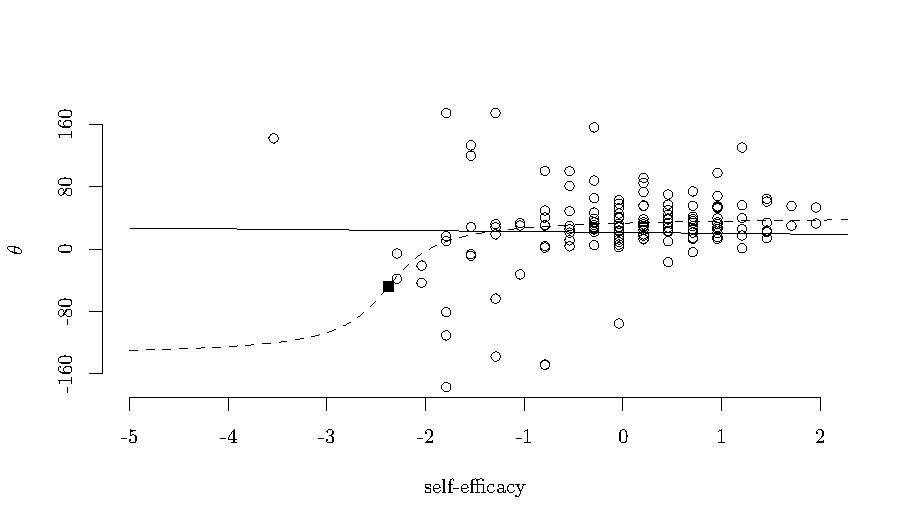
\includegraphics[width = \textwidth]{Plots/reglinediffSE.pdf}
\caption{Plot showing circular regression lines for the effect of self-efficacy
as predicted by the Abe-Ley model (solid line) and CL-PN model (dashed line). The
black square indicates the inflection point of the circular regression line for
the CL-PN model.}
\label{regline}
\end{figure}
\vspace{-0.5cm}
\subsubsection{Dependence between type and strength of interpersonal behavior.}

The relation between the type and strength of interpersonal behavior in the
CL-PN and CL-GPN models is described by the parameters \(\gamma_{\cos}\) and
\(\gamma_{\sin}\). The HPD interval of \(\gamma_{\cos}\) does not include 0 for
both the CL-PN and CL-GPN models, meaning that the cosine component of the type
of interpersonal behavior has an effect on the strength of interpersonal
behavior.\newline
\indent In the teacher data the sine and cosine components have a substantive
meaning. This is illustrated in Figure \ref{QTI}. In a unit circle the
horizontal axis (Communion) represents the cosine and the vertical axis
(Agency) represents the sine of an angle. For the teacher data this means that
the Communion (cosine) dimension of the IPC positively effects the strength of a
teachers' type of interpersonal behavior, in plain words: teachers exhibiting
interpersonal behavior types with higher communion scores (e.g., \enquote{helpful} and
\enquote{understanding} in Figure 2) are stronger in their interpersonal behavior.\newline 
\indent In the GPN-SSN model the dependence between the type and strengths of
interpersonal behavior is modelled through the covariances between the linear
outcome and the sine and cosine of the circular outcome \(\sum_{sy_{2,3}}\) and
\(\sum_{sy_{1,3}}\). Both covariances, \(\sum_{sy_{2,3}} = 0.09\) and
\(\sum_{sy_{1,3}} = 0.23\), are different from zero, but the one of the cosine
component, and thus the correlation with the Communion dimension, is larger.
This means that teachers scoring both high on Communion and Agency show stronger
behavior. Together with the results from the CL-PN and CL-GPN models in the
previous paragraph this translates to the conclusion that teachers with the
strongest interpersonal behavior have a type of interpersonal behavior between
0\(^\circ\) and 90\(^\circ\). To get these scores on the circle both the Agency and
the Communion score of a Teacher have to be positive (see \eqref{PredVal}). This
corresponds to the pattern observed in the teacher data in Figure \ref{QTI}. At
a strength of 0.4 and up we see that the scores on the circle range on average
between 0\(^\circ\) and 100\(^\circ\).

\vspace{-0.5cm}
\subsubsection{Model fit}

Table \ref{tab:ModelFit} shows the values fof the PLSL criterion for the linear
and circular outcomes of the four cylindrical models fit to the teacher
data.\newline \indent The CL-PN and CL-GPN models have the best out-of-sample
predictive performance for the linear outcome. They show roughly the same
performance because they model the linear outcome in the same way. We should
note that even though the predictive performance of the Abe-Ley model for the
linear outcome is worst on average, the standard deviation of the
cross-validation estimates is rather large. This means that in some samples, the
Abe-Ley model shows a lower PLSL value than the average of 25.49.\newline
\indent The Abe-Ley model has the best out-of-sample predictive performance for
the circular outcome. This would suggest that for the circular variable a
slightly skewed distribution fits best. However, both the GPN-SSN and the
CL-GPN models fit much worse even though the distribution for the circular
outcome in these models can also take a skewed shape. It should be noted that
the standard deviation of the cross-validation estimates is rather large for
the Abe-Ley and the CL-GPN model. It is possible that these large standard
deviations for the PLSL are caused by the fact that they are computed for a
relatively small sample size, but this does not explain why the PLSL has a large
standard deviation for only a few cylindrical models and not for all.\newline
\indent In this situation, where one model fits the linear outcome best and
another one fits the circular outcome best, it is hard to determine which model
we should choose. In this case the results for the CL-PN /CL-GPN and Abe-Ley
model are quite different regarding the effect of self-efficacy on the linear
outcome (strength of interpersonal behavior). Because the Abe-Ley fit for the
linear part is worst we would choose to trust the results for the CL-PN and
CL-GPN models here. For the circular part however the results of the CL-PN/CL-GPN
models do not differ as much from the Abe-Ley model and we reach the same
conclusion for both models, namely that the effect of self-efficacy on type of
interpersonal behavior is not very strong. Therefore we would prefer the
CL-PN/CL-GPN models in this case because where it matters in terms of
interpretation (the linear part) they show better fit.

\begin{table}

\caption{\label{tab:ModelFit}PLSL criteria, cross-validation mean and standard deviation, for the circular and linear outcome in the four cylindrical models}
\centering
\begin{tabular}[t]{lrlrl}
\toprule
\multicolumn{1}{c}{Model} & \multicolumn{2}{c}{Circular} & \multicolumn{2}{c}{Linear} \\
\cmidrule(l{2pt}r{2pt}){1-1} \cmidrule(l{2pt}r{2pt}){2-3} \cmidrule(l{2pt}r{2pt}){4-5}
  & mean & sd & mean & sd\\
\midrule
CL-PN & 82.96 & (9.47) & -17.65 & (3.70)\\
CL-GPN & 78.21 & (14.53) & -18.30 & (3.00)\\
Abe-Ley & 31.97 & (22.07) & 25.49 & (17.46)\\
GPN-SSN & 107.10 & (10.52) & -2.37 & (7.01)\\
\bottomrule
\end{tabular}
\end{table}

\vspace{-0.75cm}
\section{Discussion}\label{Discussion}
\vspace{-0.75cm}

In this paper we modified four models for cylindrical data in such a way that
they include a regression of both the linear and circular outcome onto a set of
covariates. Subsequently we have shown how these four methods can be used to
analyze a dataset on the interpersonal behavior of teachers. In this final
section we will first comment on what researchers can gain by using cylindrical
models for the teacher data. Subsequently we will comment on the differences
between the cylindrical models that were introduced in this paper.\newline
\indent Concerning the teacher data, the advantage of cylindrical data analysis
is that we were able to analyze the information about the type and strength of
interpersonal behavior simultaneously. In previous research, the two components
of the interpersonal circumplex (\emph{i.e.}, Agency and Communion) were
analyzed separately. Such an approach also provides information about the
strength of teachers' score on Agency and Communion, yet a large portion of
information about the combination of Agency and Communion, which describes the
type of behavior that is observed, gets lost. A first solution to include both
dimensions as a circular variable in data analysis was described by
Cremers et al. (2018a). A downside of that analysis was that information about
the strength of the specific type of interpersonal behavior could not be
retained. In the present study, we have shown how using cylindrical models can
simultaneously model the information about the type of and strength of
interpersonal behavior and how these are influenced by teachers' self-efficacy
in classroom management. Although we do not find any strong effects of
self-efficacy on either the type or strength of behavior, the four cylindrical
models do provide a way of analyzing and interpreting this effect. This is
beneficial for future research in which we may want to investigate the effect of
further covariates on data from the circumplex. \newline
\indent Furthermore, in addition to being able to assess the influence of
covariates, the cylindrical models also provide information about the dependence
between the type and strength of interpersonal behavior. We found that stronger
behavior is associated with higher scores on the Communion and in some models
also the Agency dimension. This implies that teachers whose type of
interpersonal behavior ranges between 0\(^\circ\) and 90\(^\circ\), the \enquote{helpful}
and \enquote{directing} subtypes are stronger in their behavior than teachers of the
other subtypes.\newline
\indent As mentioned in the introduction, data from the interpersonal circumplex
is not the only type of cylindrical data that occurs in psychology. The methods
presented in this paper are also of use for research on human navigation and
eye-tracking research. Furthermore, even though cylindrical models are already
used in fields outside of psychology, the addition of a regression structure to
the models is of use in these fields as well. \newline
\indent In terms of interpretability, the CL-PN and Abe-Ley models perform
best out of the four cylindrical models. In the
CL-GPN and GPN-SSN models the interpretation of the parameters of the
circular outcome component is not straightforward, if at all possible.
This is caused by the fact that in addition to the mean vector the
covariance matrix of the GPN distribution affects the location of the
circular data, making it difficult to compute regression coefficients on
the circle. Wang and Gelfand (2013) state that Monte Carlo integration
can be used to compute a circular mean and variance for the GPN
distribution. In future research, this solution might be applied to the
methods of Cremers et al. (2018b) in order to compute circular
coefficients for GPN models.\newline
\indent In terms of flexibility the GPN-SSN model scores best. Multiple
linear and circular outcomes can be included and we can thus apply the
model to multivariate cylindrical data. In addition the GPN-SSN, the
CL-GPN and CL-PN models are extendable to a mixed-effects structure and
can thus also be fit to longitudinal data (see Nuñez-Antonio and Gutiérrez-Peña (2014) and Hernandez-Stumpfhauser et al. (2016) for
hierarchical/mixed-effects models for the PN and GPN distributions
respectively). For the Abe-Ley model this may also be possible but has
not been done in previous research for the conditional distribution of
its circular outcome (sine-skewed von
Mises). Concerning asymmetry, both the
GPN-SSN as well as the Abe-Ley model allow for non-symmetrical shapes of
the distributions of both the linear and circular outcome, while the CL-GPN
model permits an asymmetric circular outcome.\newline
\indent The four cylindrical models that were modified to the regression
context in this paper are not the only cylindrical distributions
available from the literature. Other interesting cylindrical distributions have been introduced by
Fernández-Durán (2007), Kato and Shimizu (2008) and Sugasawa (2015) (for more references we
refer to Chapter 2 of Ley and Verdebout (2017)). In the present study we
have decided not to include these distributions for reasons of space,
complexity of the models and ease of implementing a regression
structure. In future research however it would be interesting to
investigate other types of cylindrical distributions as well in order to
compare the interpretability, flexibility and model fit to the models
developed in the present study.

\newpage
\vspace{-0.75cm}
\section*{{\normalfont References}}
\vspace{-0.75cm}

\hypertarget{refs}{}
\leavevmode\hypertarget{ref-abe2017tractable}{}%
Abe, T., \& Ley, C. (2017). A tractable, parsimonious and flexible model for cylindrical data, with applications. \emph{Econometrics and Statistics}, \emph{4}, 91--104. doi:\href{https://doi.org/10.1016/j.ecosta.2016.04.001}{10.1016/j.ecosta.2016.04.001}

\leavevmode\hypertarget{ref-chrastil2017rotational}{}%
Chrastil, E. R., \& Warren, W. H. (2017). Rotational error in path integration: Encoding and execution errors in angle reproduction. \emph{Experimental Brain Research}, \emph{235}(6), 1885--1897. doi:\href{https://doi.org/10.1007/s00221-017-4910-y}{10.1007/s00221-017-4910-y}

\leavevmode\hypertarget{ref-Claessens2016side}{}%
Claessens, L. C. (2016). \emph{Be on my side i'll be on your side : Teachers' perceptions of teacher--student relationships} (PhD thesis).

\leavevmode\hypertarget{ref-Cremers2018Assessing}{}%
Cremers, J., Mainhard, M. T., \& Klugkist, I. (2018a). Assessing a Bayesian embedding approach to circular regression models. \emph{Methodology}, \emph{14}(2), 69--81.

\leavevmode\hypertarget{ref-CremersMulderKlugkist2017}{}%
Cremers, J., Mulder, K. T., \& Klugkist, I. (2018b). Circular interpretation of regression coefficients. \emph{British Journal of Mathematical and Statistical Psychology}, \emph{71}(1), 75--95. doi:\href{https://doi.org/10.1111/bmsp.12108}{10.1111/bmsp.12108}

\leavevmode\hypertarget{ref-fernandez2007models}{}%
Fernández-Durán, J. (2007). Models for circular--linear and circular--circular data constructed from circular distributions based on nonnegative trigonometric sums. \emph{Biometrics}, \emph{63}(2), 579--585. doi:\href{https://doi.org/10.1111/j.1541-0420.2006.00716.x}{10.1111/j.1541-0420.2006.00716.x}

\leavevmode\hypertarget{ref-fisher1995statistical}{}%
Fisher, N. I. (1995). \emph{Statistical analysis of circular data}. Cambridge: Cambridge University Press.

\leavevmode\hypertarget{ref-garcia2014test}{}%
García-Portugués, E., Barros, A. M., Crujeiras, R. M., González-Manteiga, W., \& Pereira, J. (2014). A test for directional-linear independence, with applications to wildfire orientation and size. \emph{Stochastic Environmental Research and Risk Assessment}, \emph{28}(5), 1261--1275. doi:\href{https://doi.org/10.1007/s00477-013-0819-6}{10.1007/s00477-013-0819-6}

\leavevmode\hypertarget{ref-garcia2013exploring}{}%
García-Portugués, E., Crujeiras, R. M., \& González-Manteiga, W. (2013). Exploring wind direction and SO2 concentration by circular--linear density estimation. \emph{Stochastic Environmental Research and Risk Assessment}, \emph{27}(5), 1055--1067. doi:\href{https://doi.org/10.1007/s00477-012-0642-5}{10.1007/s00477-012-0642-5}

\leavevmode\hypertarget{ref-BDA}{}%
Gelman, A., Carlin, J., Stern, H., Dunson, D., Vehtari, A., \& Rubin, D. (2014). \emph{Bayesian data analysis} (3rd ed.). Boca Raton, FL: Chapman \& Hall/CRC.

\leavevmode\hypertarget{ref-gneiting2007strictly}{}%
Gneiting, T., \& Raftery, A. E. (2007). Strictly proper scoring rules, prediction, and estimation. \emph{Journal of the American Statistical Association}, \emph{102}(477), 359--378. doi:\href{https://doi.org/10.1198/016214506000001437}{10.1198/016214506000001437}

\leavevmode\hypertarget{ref-gurtman2009exploring}{}%
Gurtman, M. B. (2009). Exploring personality with the interpersonal circumplex. \emph{Social and Personality Psychology Compass}, \emph{3}(4), 601--619. doi:\href{https://doi.org/10.1111/j.1751-9004.2009.00172.x}{10.1111/j.1751-9004.2009.00172.x}

\leavevmode\hypertarget{ref-gurtman2011reasoning}{}%
Gurtman, M. B. (2011). Handbook of interpersonal psychology. In L. M. Horowitz \& S. Strack (Eds.), (pp. 299--311). New York: Wiley.

\leavevmode\hypertarget{ref-hernandez2016general}{}%
Hernandez-Stumpfhauser, D., Breidt, F. J., \& Woerd, M. J. van der. (2016). The general projected normal distribution of arbitrary dimension: Modeling and Bayesian inference. \emph{Bayesian Analysis}, \emph{12}(1), 113--133. doi:\href{https://doi.org/10.1214/15-BA989}{10.1214/15-BA989}

\leavevmode\hypertarget{ref-horowitz2010handbook}{}%
Horowitz, L. M., \& Strack, S. (2011). \emph{Handbook of interpersonal psychology: Theory, research, assessment, and therapeutic interventions}. Hoboken, NJ: John Wiley \& Sons.

\leavevmode\hypertarget{ref-jammalamadaka2001topics}{}%
Jammalamadaka, S. R., \& Sengupta, A. (2001). \emph{Topics in circular statistics} (Vol. 5). World Scientific.

\leavevmode\hypertarget{ref-johnson1978some}{}%
Johnson, R. A., \& Wehrly, T. E. (1978). Some angular-linear distributions and related regression models. \emph{Journal of the American Statistical Association}, \emph{73}(363), 602--606.

\leavevmode\hypertarget{ref-kato2008dependent}{}%
Kato, S., \& Shimizu, K. (2008). Dependent models for observations which include angular ones. \emph{Journal of Statistical Planning and Inference}, \emph{138}(11), 3538--3549. doi:\href{https://doi.org/10.1016/j.jspi.2006.12.009}{10.1016/j.jspi.2006.12.009}

\leavevmode\hypertarget{ref-lagona2015hidden}{}%
Lagona, F., Picone, M., Maruotti, A., \& Cosoli, S. (2015). A hidden Markov approach to the analysis of space--time environmental data with linear and circular components. \emph{Stochastic Environmental Research and Risk Assessment}, \emph{29}(2), 397--409. doi:\href{https://doi.org/10.1007/s00477-014-0919-y}{10.1007/s00477-014-0919-y}

\leavevmode\hypertarget{ref-leary1957}{}%
Leary, T. (1957). \emph{An interpersonal diagnosis of personality}. New York: Ronald Press Company.

\leavevmode\hypertarget{ref-ley2017modern}{}%
Ley, C., \& Verdebout, T. (2017). \emph{Modern directional statistics}. Chapman \& Hall/CRC Press. Boca Raton, FL.

\leavevmode\hypertarget{ref-locke2007selfefficacy}{}%
Locke, K. D., \& Sadler, P. (2007). Self-efficacy, values, and complementarity in dyadic interactions: Integrating interpersonal and social-cognitive theory. \emph{Personality and Social Psychology Bulletin}, \emph{33}, 94--109. doi:\href{https://doi.org/10.1177/0146167206293375}{10.1177/0146167206293375}

\leavevmode\hypertarget{ref-mardia2000directional}{}%
Mardia, K. V., \& Jupp, P. E. (2000). \emph{Directional statistics} (Vol. 494). Chichester, England: Wiley.

\leavevmode\hypertarget{ref-mardia1978model}{}%
Mardia, K. V., \& Sutton, T. W. (1978). A model for cylindrical variables with applications. \emph{Journal of the Royal Statistical Society Series B (Methodological)}, \emph{40}(2), 229--233.

\leavevmode\hypertarget{ref-mastrantonio2018joint}{}%
Mastrantonio, G. (2018). The joint projected normal and skew-normal: A distribution for poly-cylindrical data. \emph{Journal of Multivariate Analysis}, \emph{165}, 14--26. doi:\href{https://doi.org/10.1016/j.jmva.2017.11.006}{10.1016/j.jmva.2017.11.006}

\leavevmode\hypertarget{ref-mastrantonio2015bayesian}{}%
Mastrantonio, G., Maruotti, A., \& Jona-Lasinio, G. (2015). Bayesian hidden Markov modelling using circular-linear general projected normal distribution. \emph{Environmetrics}, \emph{26}(2), 145--158. doi:\href{https://doi.org/10.1002/env.2326}{10.1002/env.2326}

\leavevmode\hypertarget{ref-nunez2014bayesian}{}%
Nuñez-Antonio, G., \& Gutiérrez-Peña, E. (2014). A Bayesian model for longitudinal circular data based on the projected normal distribution. \emph{Computational Statistics \& Data Analysis}, \emph{71}, 506--519. doi:\href{https://doi.org/10.1016/j.csda.2012.07.025}{10.1016/j.csda.2012.07.025}

\leavevmode\hypertarget{ref-nunez2011bayesian}{}%
Nuñez-Antonio, G., Gutiérrez-Peña, E., \& Escarela, G. (2011). A Bayesian regression model for circular data based on the projected normal distribution. \emph{Statistical Modelling}, \emph{11}(3), 185--201. doi:\href{https://doi.org/10.1177/1471082X1001100301}{10.1177/1471082X1001100301}

\leavevmode\hypertarget{ref-pennings2017phd}{}%
Pennings, H. J. M. (2017a). \emph{Interpersonal dynamics in teacher-student interactions and relationships} (PhD thesis). Enschede: Ipskamp drukkers.

\leavevmode\hypertarget{ref-pennings2017complexity}{}%
Pennings, H. J. M. (2017b). Using a complexity approach to study the interpersonal dynamics in teacher-student interactions: A case study of two teachers. \emph{Complicity: An International Journal of Complexity and Education}, \emph{14}(2), 88--103.

\leavevmode\hypertarget{ref-pennings2018interpersonal}{}%
Pennings, H. J. M., Brekelmans, M., Sadler, P., Claessens, L. C., \VANDER{Want}{Van der}{van der} Want, A. C., \& \VAN{Tartwijk}{Van}{van} Tartwijk, J. (2018). Interpersonal adaptation in teacher-student interaction. \emph{Learning and Instruction}, \emph{55}, 41--57. doi:\href{https://doi.org/10.1016/j.learninstruc.2017.09.005}{10.1016/j.learninstruc.2017.09.005}

\leavevmode\hypertarget{ref-plutchik1997general}{}%
Plutchik, R. (1997). Circumplex models of personality and emotions. In C. Plutchik Robert. (Ed.), (pp. 17--45). Washington, DC, US: American Psychological Association.

\leavevmode\hypertarget{ref-rayner200935th}{}%
Rayner, K. (2009). The 35th Sir Frederick Bartlett lecture: Eye movements and attention in reading, scene perception, and visual search. \emph{Quarterly Journal of Experimental Psychology}, \emph{62}(8), 1457--1506. doi:\href{https://doi.org/10.1080/17470210902816461}{10.1080/17470210902816461}

\leavevmode\hypertarget{ref-russell1980circumplex}{}%
Russell, J. A. (1980). A circumplex model of affect. \emph{Journal of Personality and Social Psychology}, \emph{39}(6), 1161--1178. doi:\href{https://doi.org/10.1037/h0077714}{10.1037/h0077714}

\leavevmode\hypertarget{ref-sahu2003new}{}%
Sahu, S. K., Dey, D. K., \& Branco, M. D. (2003). A new class of multivariate skew distributions with applications to Bayesian regression models. \emph{Canadian Journal of Statistics}, \emph{31}(2), 129--150. doi:\href{https://doi.org/10.2307/3316064}{10.2307/3316064}

\leavevmode\hypertarget{ref-schwartz1992values}{}%
Schwartz, S. H. (1992). Advances in experimental social psychology. In M. Zanna (Ed.), (Vol. 25, pp. 1--65). San Diego, CA: Academic Press.

\leavevmode\hypertarget{ref-sugasawa2015flexible}{}%
Sugasawa, S., S. (2015). \emph{A flexible family of distributions on the cylinder}. Retrieved from \href{arXiv:\%201501.06332v2}{arXiv: 1501.06332v2}

\leavevmode\hypertarget{ref-wang2012directional}{}%
Wang, F., \& Gelfand, A. E. (2013). Directional data analysis under the general projected normal distribution. \emph{Statistical Methodology}, \emph{10}(1), 113--127. doi:\href{https://doi.org/10.1016/j.stamet.2012.07.005}{10.1016/j.stamet.2012.07.005}

\leavevmode\hypertarget{ref-vanderWant2015role}{}%
\VANDER{Want}{Van der}{van der} Want, A. C. (2015). \emph{Teachers' interpersonal role identity.} (PhD thesis).

\leavevmode\hypertarget{ref-want2018selfefficacy}{}%
\VANDER{Want}{Van der}{van der} Want, A. C., \DEN{Brok}{Den}{den} Brok, P., Beijaard, D., Brekelmans, M., Claessens, L. C., \& Pennings, H. J. M. (2018). The relation between teachers' interpersonal role identity and their self-efficacy, burnout and work engagement. \emph{Professional Development in Education}, Advance Online Publication. doi:\href{https://doi.org/10.1080/19415257.2018.1511453}{10.1080/19415257.2018.1511453}

\leavevmode\hypertarget{ref-wiggins1996history}{}%
Wiggins, J. (1996). An informal history of the interpersonal circumplex tradition. \emph{Journal of Personality Assessment}, \emph{66}(2), 217--233.

\leavevmode\hypertarget{ref-wright2009integrating}{}%
Wright, A. G., Pincus, A. L., Conroy, D. E., \& Hilsenroth, M. J. (2009). Integrating methods to optimize circumplex description and comparison of groups. \emph{Journal of Personality Assessment}, \emph{91}(4), 311--322. doi:\href{https://doi.org/10.1080/00223890902935696}{10.1080/00223890902935696}

\leavevmode\hypertarget{ref-wubbels2006interpersonal}{}%
Wubbels, T., Brekelmans, M., \DEN{Brok}{Den}{den} Brok, P., \& \VAN{Tartwijk}{Van}{van} Tartwijk, J. (2006). Handbook of classroom management: Research practice and contemporary issues. In C. Evertson \& C. S. Weinstein (Eds.), \emph{Handbook of classroom management: Research, practice, and contemporary issues} (pp. 1161--1191). Malwah, NJ: Lawrence Erlbaum Associates.


\end{document}
